\DeclareUnicodeCharacter{FB01}{fi}
\DeclareUnicodeCharacter{FB02}{fi}
%%%%%%%%%%%%%%%%%%%%%%%%%%%%%%%%%%%%%%%%%
% Masters/Doctoral Thesis 
% LaTeX Template
% Version 2.5 (27/8/17)
%
% This template was downloaded from:
% http://www.LaTeXTemplates.com
%
% Version 2.x major modifications by:
% Vel (vel@latextemplates.com)
%
% This template is based on a template by:
% Steve Gunn (http://users.ecs.soton.ac.uk/srg/softwaretools/document/templates/)
% Sunil Patel (http://www.sunilpatel.co.uk/thesi -template/)
%
% Template license:
% CC B -N -SA 3.0 (http://creativecommons.org/licenses/b -n -sa/3.0/)
%
%%%%%%%%%%%%%%%%%%%%%%%%%%%%%%%%%%%%%%%%%


%	PACKAGES AND OTHER DOCUMENT CONFIGURATIONS


\documentclass[
12pt, % The default document font size, options: 10pt, 11pt, 12pt
oneside, % Two side (alternating margins) for binding by default, uncomment to switch to one side
english, % ngerman for German
doublespacing, % Single line spacing, alternatives: onehalfspacing or doublespacing
%draft, % Uncomment to enable draft mode (no pictures, no links, overfull hboxes indicated)
nolistspacing, % If the document is onehalfspacing or doublespacing, uncomment this to set spacing in lists to single
liststotoc, % Uncomment to add the list of figures/tables/etc to the table of contents
toctotoc, % Uncomment to add the main table of contents to the table of contents
parskip, % Uncomment to add space between paragraphs
%nohyperref, % Uncomment to not load the hyperref package
headsepline, % Uncomment to get a line under the header
chapterinoneline, % Uncomment to place the chapter title next to the number on one line
consistentlayout, % Uncomment to change the layout of the declaration, abstract and acknowledgements pages to match the default layout
]{MastersDoctoralThesis} % The class file specifying the document structure

\usepackage[utf8]{inputenc} % Required for inputting international characters
\usepackage[T1]{fontenc} % Output font encoding for international characters

\usepackage{mathpazo} % Use the Palatino font by default

\usepackage[backend=bibtex,
bibstyle=numeric,
citestyle=numeric-comp,
natbib=true,hyperref=true,sorting=ynt]{biblatex} % Use the bibtex backend with the authoryear citation style (which resembles APA)

\addbibresource{MyLibrary.bib} % The filename of the bibliography

\usepackage[autostyle=true]{csquotes} % Required to generate languag -dependent quotes in the bibliography

\usepackage{float} 
\usepackage{aligned-overset}
\usepackage{amssymb}
\usepackage[utf8]{inputenc}

%	MARGIN SETTINGS


\geometry{
	paper=a4paper, % Change to letterpaper for US letter
	inner=2cm, % Inner margin
	outer=2cm, % Outer margin
	bindingoffset=0cm, % Binding offset
	top=1.3cm, % Top margin
	bottom=1.3cm, % Bottom margin
	%showframe, % Uncomment to show how the type block is set on the page
}


%	THESIS INFORMATION


\thesistitle{Single-cell Trajectory Inference Approaches} % Your thesis title, this is used in the title and abstract, print it elsewhere with \ttitle
\supervisor{Prof. Wei \textsc{Huang}} % Your supervisor's name, this is used in the title page, print it elsewhere with \supname
%\examiner{huhuhuhu} % Your examiner's name, this is not currently used anywhere in the template, print it elsewhere with \examname
\degree{Literature Review} % Your degree name, this is used in the title page and abstract, print it elsewhere with \degreename
\author{Siyuan \textsc{Guo} 11611118 } % Your name, this is used in the title page and abstract, print it elsewhere with \authorname
\addresses{Shenzhen} % Your address, this is not currently used anywhere in the template, print it elsewhere with \addressname

\subject{Biological Sciences} % Your subject area, this is not currently used anywhere in the template, print it elsewhere with \subjectname
\keywords{} % Keywords for your thesis, this is not currently used anywhere in the template, print it elsewhere with \keywordnames
\university{\href{http://www.university.com}{Southern University of Science and Technology}} % Your university's name and URL, this is used in the title page and abstract, print it elsewhere with \univname
\department{\href{http://department.university.com}{Department of Biology}} % Your department's name and URL, this is used in the title page and abstract, print it elsewhere with \deptname
\group{\href{http://researchgroup.university.com}{BIO302}} % Your research group's name and URL, this is used in the title page, print it elsewhere with \groupname
%\faculty{\href{http://faculty.university.com}{Faculty Name}} % Your faculty's name and URL, this is used in the title page and abstract, print it elsewhere with \facname

\AtBeginDocument{
\hypersetup{pdftitle=\ttitle} % Set the PDF's title to your title
\hypersetup{pdfauthor=\authorname} % Set the PDF's author to your name
\hypersetup{pdfkeywords=\keywordnames} % Set the PDF's keywords to your keywords
}

\begin{document}

\frontmatter % Use roman page numbering style (i, ii, iii, iv...) for the pr - content pages

\pagestyle{plain} % Default to the plain heading style until the thesis style is called for the body content


%	TITLE PAGE


\begin{titlepage}
\begin{center}

\vspace*{.06\textheight}
{\scshape \LARGE \univname \par}\vspace{1.0cm} % University name
\textsc{\Large BIO304: SYSTEMS BIOLOGY}\\[0.5cm] % Thesis type

\HRule \\[0.56cm] % Horizontal line
{\huge \bfseries \ttitle \par}\vspace{0.5cm} % Thesis title
\HRule \\[0.8cm] % Horizontal line
 
\begin{minipage}[t]{0.4\textwidth}
\begin{flushleft} \large
\emph{Author:}\\
\href{http://www.johnsmith.com}{\authorname} % Author name - remove the \href bracket to remove the link
\end{flushleft}
\end{minipage}
\begin{minipage}[t]{0.4\textwidth}
\begin{flushright} \large
\emph{Supervisor:} \\
\href{http://www.jamessmith.com}{\supname} % Supervisor name - remove the \href bracket to remove the link  
\end{flushright}
\end{minipage}\\[5cm]

\Large \deptname\\[0cm] % Research group name and department name
 
{\large \today}\\[0cm] % Date
%\includegraphics{Logo} % University/department logo - uncomment to place it
 
\end{center}
\end{titlepage}


\begin{abstract}
\addchaptertocentry{\abstractname} 
Since the discovery of the cell in 1665, scientists have been working to classify cells and build cell lineage. In the process, scientists have developed a variety of methods and made some great achievements. In recent years, single-cell sequencing technology has developed rapidly, and researchers have developed a number of single-cell trajectory inference tools that can use single-cell sequencing data to classify cells and build cell lineage, turning research of cellular dynamic processes into analysis of the pseudo-time series and greatly improved analysis throughput. Some ambitious scientists also hope to use this technology to construct “The Human Cell Atlas”. The existing scTI methods have achieved many achievements. In some simple cell differentiation systems, scientists have used these methods to find answers to many important biological problems. The paper also lists 20 commonly used scTI methods and 7 basic topologies in the cell lineage, and organizes and summarizes the basic information of these methods and their adaptability to various basic topologies. At the same time, in fact, cell lineage studies based on single-cell biology are still in the early stages of development, and scientists need more powerful sequencing techniques and better-performing core algorithms to further develop these scTI research strategies. In future biological research, especially after scientists have successfully mapped the complete “The Human Cell Atlas” and the cell lineage of various model animals, single-cell-based cell lineage and classification studies will provide a powerful boost to the development of biology.
\end{abstract}

\tableofcontents

\mainmatter % Begin numeric (1,2,3...) page numbering

\pagestyle{thesis} % Return the page headers back to the "thesis" style

% Include the chapters of the thesis as separate files from the Chapters folder
% Uncomment the lines as you write the chapters

%------------------------ ---------------------------------------------------------------

% Define some commandsx to keep the formatting separated from the content 
\newcommand{\keyword}[1]{\textbf{#1}}
\newcommand{\tabhead}[1]{\textbf{#1}}
\newcommand{\code}[1]{\texttt{#1}}
\newcommand{\file}[1]{\texttt{\bfseries#1}}
\newcommand{\option}[1]{\texttt{\itshape#1}}

%----------------------------------------------------------------------------------------

\chapter{Background} % Main chapter title

\label{Background} % For referencing the chapter elsewhere, use \ref{Chapter1} 

\section{Cell}

Modern biology theory defines the cells discovered by Hooke in 1665 as the most basic unit of organic organisms. Modern cell theory consists of three parts, all living things are composed of cells and cell products; cells are the most basic unit of life structure and function; all new cells are derived from old cells.

\subsection{Cell Lineage}

Cell lineage refers to the developmental history of blastomeres from the time of the first cleavage until the final differentiation into tissues and organ cells. The division of fertilized eggs in many animals is carried out in a strict format. In this process, the moment, the order, and the location in the space of the splitting balls' generation are specified. This kind of inter-cell relationship in the developmental generation is like the lineage of the human family, so it is called the cell lineage \parencite{regev_human_2017,nowogrodzki_how_2017}. \\

The study of cell lineage plays an important role in understanding the relationship between the uneven distribution of egg quality and the developmental fate of blastomeres, as well as the evolutionary relationship between the early development of different species of animals. In the past many years, researchers have also begun to focus on the pedigree research of abnormal developmental cells such as cancer cells, in order to systematically understand its occurrence process and mechanism \parencite{regev_human_2017}.

\subsection{Cell Classification}

For a long time, scientists have been working to discover and classify a wide variety of cells. At the same time, they are also committed to a detailed description of the characteristics of each cell type. However, due to the limitations of technology, scientists can only distinguish different types of cells by their shape, their position in the organism and their relative relationship with other cells. \\

After various chemical stains were discovered, scientists began to classify and differentiate them using the performance of various cells under different stains. The 1906 Nobel Prize in Physiology or Medicine was awarded to two scientists who used staining techniques and anatomical techniques to study the diverse structures of the brain. \\

Due to the imaging limitations of optical microscopy, in order to better study cell structure and other characteristics, scientists began to seek more powerful microscopic imaging tools. Since the 1930s, electron microscopy, which has been able to provide imaging magnifications of up to 5000 times, has become one of the important tools for biological research. In the rapid development phase of subsequent science, various modern biotechnologies such as FACS (fluorescence activated cell sorting) and FISH (fluorescence in situ hybridization) help researchers distinguish various cell types. \\

Today, we have so many techniques and methods to classify cells, and it seems that scientists are about to realize their ultimate pursuit of cell sorting. But the facts are not always satisfactory. In fact, the various results we have achieved on cell classification can only be considered to be fragmented and one-sided. The various classification models we have are often based on different detection indicators and evaluation criteria, and the correlation between these indicators is difficult to be strictly defined and evaluated, so the integration of different classification models becomes an extremely difficult task. So far, we have established a complete cell lineage of fertilized eggs to mature bodies only in $C. elegan$. It is a kind of extremely simple creature and its mature individuals have only about 1000 cells. At the same time, the number of cells in different mature individuals of the same sex is the same. This is a rare character which is very meaningful in building cell lineage. \\

At the same time, due to the confusion of various detection methods and evaluation methods, we lack a strict definition of some basic concepts in the cell classification problem, which may cause confusion and trouble in some cases. The booming single-cell omics technology in recent years provides researchers with a comprehensive set of comprehensive indicators. Many researchers believe that this set of techniques can provide data-based definitions for different cell types, which greatly increases the accuracy of the definition. Also, single-cell multi-omics technology provides a platform on which scientists can re-integrate the various cell maps we know into a huge one with adding more single-cell level details to it. And they can also find that some cell types and cell development pathways which have not been discovered. 

\section{Single-cell Biology and Cell Lineage}

\subsection{Single-cell Omics}

As one of the most basic unit concepts of life, cells are the cornerstone of life activities. Although biologists have been working under a microscope for nearly 180 years, we still don't know much about cells. We expect effective technical means to completely examine the composition of individual cells to identify and treat diseases at the cellular and even molecular levels \parencite{noauthor_single-cell_2017, perkel_single-cell_2017}. \\

Single-cell sequencing refers to the technique of obtaining data and analyzing information by sequencing the levels of genomes, transcriptomes and epigenetic-genomes of individual cells. Single-cell sequencing can solve the problem of cellular heterogeneity that cannot be solved by traditionally sequencing mixed tissue samples, and provides a new method for analyzing the behavior, mechanism and relationship between individual cells and the body 
\parencite{perkel_single-cell_2017,regev_human_2017}. \\

In conventional tissue RNA sequencing methods, the signals produced by different kinds of cells are averaged. Throughout the process, the difference between cells and cells, also known as cytoplasmic heterogeneity, was ignored. We can't find two identical cells in nature, and scRNA-seq provides us with the opportunity to discover the tiny differences between these cells. Using a scRNA-seq data-driven approach, researchers also have the chance to discover some new cell types \parencite{regev_human_2017}. Single-cell genome and epigenetic genome sequencing can identify cell genomes. The purpose of the genome approach is to identify the entire genome or capture a specific predefined region. Epigenetic methods can capture specific predefined sequences based on unique histone modification (scChIP-Seq), genome openness (scATAC-Seq), or the same identification of DNA methylation patterns (scDNAme-Seq) or 3D chromosome-structures (scHi-C) \parencite{nowogrodzki_how_2017}. A combination of barcode-strategies is now used to capture tens of thousands of single cells. Single-cell epigenetic genomics methods usually study only the nucleus, so frozen or certain fixed samples could be used. 
 
\subsection{The Human Cell Atlas}

Scientists have long recognized the need for a deeper understanding of cells, but until recently, with the rapid development of single-cell omics technology, the creation of a complete and systematic human cell map has become a viable goal. In 2017, researchers from different countries proposed an initiative to open a project called ``The Human Cell Atlas'' 
\parencite{regev_human_2017}. This is an ambitious project that, like the Human Genome Project, attempts to provide data support for fundamentally solving biological problems. 

\subsection{Single-cell Trajectory Inference (scTI)}

In traditional studies of cellular dynamic processes (such as cell cycle, cell differentiation, and cell activation), scientists rely mainly on tracking cells calibrated in multiple sets of parallel experiments at different time nodes, a method that is undoubtedly very complex and time-consuming. Cells reach the cell types they  finally differentiate to by distinguishing between asynchronous branching pathways. The material basis of this differentiation process is the change of molecular characteristics within cells, especially the regulation of different gene expression levels by cells at different times. The method based on single-cell omics (such as transcription, proteomics, and epigenetic genomics) is actually a pseudo-time sequence analysis strategy, which means that researchers can analyze the entire cellular dynamic process with few static samples \parencite{tanay_scaling_2017,etzrodt_quantitative_2014}. \\

These dynamic process can be inferred by a trajectory inference (TI) method \parencite{regev_human_2017, nowogrodzki_how_2017}. It sorts cells along the trajectory according to the similarity of cell expression patterns. Through this technique, single cell cytology can reconstruct the evolution process of cells into a trajectory of high-dimensional space 
\parencite{trapnell_defining_2015,cannoodt_computational_2016,moon_manifold_2018}. In general, trajectories produced by this method are linear, tree-shaped or bifurcated. But some of the latest methods also support the formation of trajectories consisting of more complex topologies, such as ring structures 
\parencite{liu_reconstructing_2017} and structures containing broken connections 
\parencite{wolf_paga:_2019}. TI methods can help us to fully understand the dynamics of cells from a single-cell omics perspective \parencite{tanay_scaling_2017}, objectively identify different cell subtypes and subsets of cells \parencite{schlitzer_identification_2015} and map the corresponding cell differentiation trees \parencite{velten_human_2017,see_mapping_2017}, and infer cell-cell interactions regulating differentiation bifurcations between cells 
\parencite{aibar_scenic:_2017}. \\

If researchers had large enough single-celled sample sets, they would also have the opportunity to discover phenomena that could not be observed in normal cellular development dynamics systems. The more complex the cell lineage path, the more intersections there are, the larger the sample set is needed to study the above anomalies. At the same time, reasonable selection of clustering or regression algorithm to classify cells is beneficial for researchers to observe rare cell intermediate states and cell subtypes. When the cellular lineage of the entire sample set is constructed, researchers can analyze the distribution of cells on different pathways along the lineage direction to obtain the relative duration and clustering size of each cell development stage, and analyze the subset of progenitor cells in the whole dataset 
\parencite{regev_human_2017}. 



%----------------------------------------------------------------------------------------
%\newpage






%----------------------------------------------------------------------------------------







%----------------------------------------------------------------------------------------



%----------------------------------------------------------------------------------------




%The \code{biblatex} package is used to format the bibliography and inserts references such as this one \parencite{Reference1}. The options used in the \file{main.tex} file mean that the in-text citations of references are formatted with the author(s) listed with the date of the publication. Multiple references are separated by semicolons (e.g. \parencite{Reference2, Reference1}) and references with more than three authors only show the first author with \emph{et al.} indicating there are more authors (e.g. \parencite{Reference3}). This is done automatically for you. To see how you use references, have a look at the \file{Chapter1.tex} source file. Many reference managers allow you to simply drag the reference into the document as you type.

 
\chapter{Modeling doxycycline-induced mCherry expression systems, with feedback} % Main chapter title

\label{Part2_chapter} % For referencing the chapter elsewhere, use \ref{Chapter1} 



\section{Informations}

1. pCMV is a constitutive promoter.

2. Black triangle is a tetR-dimer binding site (tetO), there are two of them near TATA box

3. NLS is nuclear localization sequence, facilitate the translocation of tetR to nucleus.

4. In the absence of Doxcycline, tetR-dimer preferably binds to tetO, block the RNA polymerase.

5. In the presence of Doxcycline, tetR-dimer preferably disassociate from tetO, remove the interference to RNA polymerase.

\begin{figure}[th]
\centering
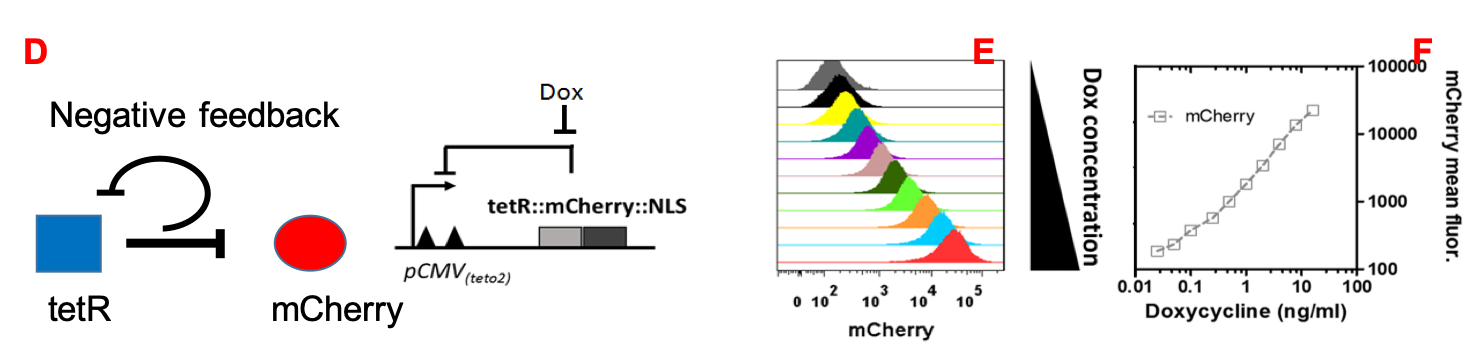
\includegraphics[width=1.0\linewidth]{Figures/part2.png}
\caption{Pictures of part 2}
\label{part_2_qestion_figure}
\end{figure}
%----------------------------------------------------------------------------------------
\section{Write step-by-step reactions}

\subsection{Symbols}

\begin{table}[H]
\caption{Modeling doxycycline-induced mCherry expression systems with feedback}
\label{tab:part2_symbols}
\centering
\begin{tabular}{l l}
\toprule

\tabhead{Symbol} & \tabhead{Definition} \\
\midrule
$D$ & The doxycycline molecular\\
$R$ & The tetR molecular\\
$R^{2}_{i}$ &   % ${\rm R^{2}_{i}}$ 改成正常体
The tetR-dimer molecular binds with \keyword{i} doxycycline molecular \\
$R^2$ & 
A mixture of $R^{2}_{0}$, $R^{2}_{1}$ and $R^{2}_{2}$\\
$O_{m}$ & 
The $tetO^{2}$ binding with m $R^{2}_{0}(m = 0, 1, 2)$\\
%\quad$O_{00}$ & 
%\quad Both two tetOs are free \\
%\quad$O_{10}$ & 
%\quad One tetO is free and another is occupied by $R^{2}_{1}$ \\
%\quad$O_{11}$ & 
%\quad Both two tetOs are occupied by $R^{2}_{1}$ \\
%\quad$O_{20}$ & 
%\quad One tetO is free and another is occupied by $R^{2}_{0}$ \\
%\quad$O_{21}$ & 
%\quad Two tetO are respectively occupied by a $R^{2}_{0}$ and a $R^{2}_{1}$\\
%\quad$O_{22}$ & 
%\quad Both two tetOs are occupied by $R^{2}_{0}$ \\
$O_{on}$ & 
The binding situation of $tetO^{2}$ that turn on the expression of GFP mRNA\\
$O_{sum}$ & 
Including $O_{0}, O_{1}, O_{2}$ \\
$C$ & 
mCherry protein \\
$P$ & 
RNA polymerase \\
$K_{1}$ & 
Reaction equilibrium constant of $R^{2}_{0}$ formation from $R$\\
$K_{2}$ & 
Reaction equilibrium constant of $R^{2}_{1}$ formation from $R^{2}_{0}$\\
$\sigma_{1}$ & 
$K_{3} = \sigma_{1} K_{2}$, \\ &so $\sigma_{1}$ represent binding strengths relative to the tetR-dimer-$tetO^{2}$ strength \\
$K_{3}$ & 
Reaction equilibrium constant of $R^{2}_{2}$ formation from $R^{2}_{1}$\\
$K_{4}$ & 
Reaction equilibrium constant of $O_{1}$ formation from $O_{0}$\\
$\sigma_{2}$ & 
$K_{5} = \sigma_{2} K_{4}$, \\ &so $\sigma_{2}$ represent binding strengths relative to the tetR-dimer-doxycycline strength \\
$K_{5}$ & 
Reaction equilibrium constant of $O_{2}$ formation from $O_{1}$\\
$k_{t}$ & 
Reaction constant of mCherry and tetR production\\
$k_{d-c}$ & 
Reaction constant of mCherry degradation\\
$k_{d-rd}$ & 
Reaction constant of tetR-dimer degradation\\
$P_{0}$ & 
I assume that the concentration of $P$ remains constant as $P_{0}$ during time\\
$n_c$ & 
The number of mCherry per mRNA transcript\\
$n_{rd}$ & 
The number of tetR-dimer per mRNA transcript\\
$r_c$ & 
The basal rate of production of mCherry\\
$r_{rd}$ & 
The basal rate of production of tetR-dimer\\
\bottomrule\\
\end{tabular}
\end{table}
\newpage


\subsection{Model}
The chemical reactions describing the network are naturally divided into two categories—fast and slow. The fast reactions have rate constants of order seconds and are therefore assumed to be in equilibrium with respect to the slow reactions, which are described by rates of order minutes.

Considering the reactions between tetR molecular, tetR-dimer molecular and doxycycline molecular, then we may write the equilibrium fast reactions :

\begin{equation} 
\begin{aligned} 
\centering
% \underset{A}{B}
% \overset{…}{…}
2R         &\underset{}{\overset{K_1}{\rightleftharpoons}} R^2_0 \\ 
R^2_0 + D  &\underset{}{\overset{K_2}{\rightleftharpoons}} R^2_1 \\ 
R^2_1 + D  &\underset{}{\overset{K_3}{\rightleftharpoons}} R^2_2 \\  
\end{aligned} 
\end{equation}

If we ignore the exsit of tetR molecular and assume all of them will take part in the formation of tetR-dimer molecular, in aother word, the $K_1$ is extrimly huge, the reactions become : 

\begin{equation} 
\begin{aligned} 
\centering
% \underset{A}{B}
% \overset{…}{…}
R^2_0 + D  &\underset{}{\overset{K_2}{\rightleftharpoons}} R^2_1 \\ 
R^2_1 + D  &\underset{}{\overset{K_3}{\rightleftharpoons}} R^2_2 \\  
\end{aligned} 
\end{equation}

Considering the reactions between tetR-dimer molecular and $tetO^{2}$, and it is assumed that the tetR-dimer binding with doxycycline molecular could not binding to $tetO^{2}$, then we may write the equilibrium fast reactions :

\begin{equation} 
\begin{aligned} 
\centering
% \underset{A}{B}
% \overset{…}{…}
O_0 + R^2_0  &\underset{}{\overset{K_4}{\rightleftharpoons}} O_1 \\ 
O_1 + R^2_0  &\underset{}{\overset{K_5}{\rightleftharpoons}} O_2 \\  
\end{aligned} 
\end{equation}

It is assumed that only $O_0$ can bind to $tetO^{2}$. \\
The slow reactions are transcription and degradation :

\begin{equation} 
\centering
\begin{aligned} 
% \underset{A}{B}
% \overset{…}{…}
\qquad \qquad \quad[O_{on}]    &= [O_0] \\
%\qquad \qquad \quad[O_{on}]    &= [O_0] + \frac{1}{2}[O_1] \\
\qquad \qquad \quad O_{on} + P &\underset{}{\overset{k_t}{\rightarrow}} 
O_{on} + P + n_cC + n_{rd}R^2\\ 
\qquad \qquad \quad C          &\underset{}{\overset{k_{d-c}}{\rightarrow}} 
\phi \\  
\qquad \qquad \quad R^2      &\underset{}{\overset{k_{d-rd}}{\rightarrow}} 
\phi \\  
\end{aligned} 
\end{equation}

The number of $tetO^{2}$ is depended by the number of plasmids in the cell. So the number of $tetO^{2}$ is a constant, which means $O_{sum}$ = $[O_0]+[O_1]+[O_2]$ does not change in a specific cell. Also, since the transcription reaction is slower than the reactions in Eq.2.1, the $R_0^2$ produced in transcription will partly become $R_1^2$ and $R_2^2$. So $R^2$ was used to donate this mixture of $R_0^2$, $R_1^2$ and $R_2^2$. $[R^2]$ = $[R_0^2]$ + $[R_1^2]$ + $[R_2^2]$

\subsection{Reactions}

\begin{equation*} 
\begin{aligned} 
\centering
% \underset{A}{B}
% \overset{…}{…}
R^2_0 + D    &\underset{}{\overset{K_2}{\rightleftharpoons}} R^2_1 \\ 
R^2_1 + D    &\underset{}{\overset{K_3}{\rightleftharpoons}} R^2_2 \\  
O_0 + R^2_0  &\underset{}{\overset{K_4}{\rightleftharpoons}} O_1 \\ 
O_1 + R^2_0  &\underset{}{\overset{K_5}{\rightleftharpoons}} O_2 \\ 
[O_{on}]     &= [O_0] \\
O_{on} + P   &\underset{}{\overset{k_t}{\rightarrow}} O_{on} + P + n_cC + n_{rd}R^2\\
C            &\underset{}{\overset{k_{d-c}}{\rightarrow}} \phi \\  
R^2        &\underset{}{\overset{k_{d-rd}}{\rightarrow}} \phi \\  
\end{aligned} 
\end{equation*}


%----------------------------------------------------------------------------------------

\section{Write ODE equations from reactions}

Form the reactions above, ODE equations could be written and we know that : 
\begin{equation} 
\begin{aligned} 
\centering
% \underset{A}{B}
% \overset{…}{…}
K_i &= \frac{k_i}{k_{-i}}(i = 2,3,4,5) \\
\frac{d[R_0^2]}{dt} &=  + k_{-2} [R^2_1] + k_{-4}[O_1] + k_{-5}[O_2] \\
				    &\qquad - (k_2[D]+k_4[O_0]+k_5[O_1]) [R_0^2] \\
\frac{d[R_1^2]}{dt} &= k_{-3}[R_2^2]-k_3[R^2_1][D]+k_2[R^2_0][D]-k_{-2}[R^2_1] \\
\frac{d[R_2^2]}{dt} &= k_{3}[R_2^1][D]- k_{-3}[R^2_2] \\
\frac{d[O_0]}{dt} &= k_{-4}[O_1]-k_4[O_0][R_0^2] \\
\frac{d[O_1]}{dt} &= k_4[O_0][R_0^2]-k_{-4}[O_1]+k_{-5}[O_2]-k_5[O_1][R_0^2] \\
\frac{d[O_2]}{dt} &= k_5[O_1][R_0^2]-k_{-5}[O_2] \\
\frac{d[C]}{dt} &= n_c k_t P_0 [O_0] - k_{d-c}[C] + r_c \\
\frac{d[R^2]}{dt} &= n_{rd} k_t P_0 [O_0] - k_{d-rd}[R^2] + r_{rd} \\
[R^2] &= [R_0^2] + [R_1^2] + [R_2^2]
%[O_{on}]     &= [O_0] \\
%[O_{on}]     &= [O_0] + \frac{1}{2}[O_1] \\
\end{aligned} 
\end{equation}

%----------------------------------------------------------------------------------------
\newpage
\section{Simplified the model with quasi-steady state assumption and justified the assumptions}

\subsection{Simplification}
Reaction in Eq.2.2 and Eq.2.3 can be simplified as steady-state.
So I get the equations :

\begin{equation} 
\begin{aligned} 
\centering
% \underset{A}{B}
% \overset{…}{…}
[R^2_1] &= K_2[D][R^2_0] \\
[R^2_2] &= K_3[D][R^2_1] \\
[O_1]   &= K_4[R^2_0][O_0] \\
[O_2]   &= K_5[R^2_0][O_1] \\
K_{3} &= \sigma_{1} K_{2} \\
K_{5} &= \sigma_{2} K_{4} \\
\end{aligned} 
\end{equation}

Then these equations could be written as:
\begin{equation} 
\begin{aligned} 
\centering
% \underset{A}{B}
% \overset{…}{…}
[R^2_1] &= K_2[D][R^2_0] \\
[R^2_2] &= \sigma_{1}K_2^2[D]^2[R^2_0] \\
[O_1]   &= K_4[R^2_0][O_0] \\
[O_2]   &= \sigma_{2}K_4^2[R^2_0]^2[O_0] \\
O_{sum} &= [O_0]+[O_1]+[O_2] \\
\end{aligned} 
\end{equation}

From Eq.2.4 we can get ODE equations : 

\begin{equation} 
\begin{aligned} 
\centering
\frac{d[C]}{dt} &= n_c k_t P_0 [O_0] - k_{d-c}[C] + r_c \\
\frac{d[R^2]}{dt} &= n_{rd} k_t P_0 [O_0] - k_{d-rd}[R^2] + r_{rd} \\
[R^2] &= [R_0^2] + [R_1^2] + [R_2^2]
\end{aligned} 
\end{equation}

Then these equations could be written as :
\begin{equation} 
\begin{aligned} 
\centering
\frac{d[C]}{dt} &= n_c k_t P_0 [O_0] - k_{d-c}[C] + r_c \\
\frac{d[R^2_0]}{dt} &= \frac{n_{rd}k_tP_0[O_0]}{1+K_2[D]+\sigma_1K_2^2[D]^2} 
- k_{d-rd}[R^2_0] + \frac{r_{rd}}{1+K_2[D]+\sigma_1K_2^2[D]^2} \\
\end{aligned} 
\end{equation}

Using $O_{sum}$ to present $[O_0]$ :
\begin{equation} 
\begin{aligned} 
\centering
\frac{d[C]}{dt} &= \frac{n_c k_t P_0 O_{sum}}{1+K_4[R_0^2]+\sigma_2 K_4^2 [R_0^2]^2} 
- k_{d-c}[C] + r_c \\
\frac{d[R^2_0]}{dt} &= 
\frac{n_{rd} k_t P_0 O_{sum}}
{(1+K_2[D]+\sigma_1K_2^2[D]^2)(1+K_4[R_0^2]+\sigma_2 K_4^2 [R_0^2]^2)}\\ 
&\qquad - k_{d-rd}[R^2_0] + \frac{r_{rd}}{1+K_2[D]+\sigma_1 K_2^2 [D]^2} \\
\end{aligned} 
\end{equation}


 
Then: 
\begin{equation} 
\begin{aligned} 
           \alpha_1 &= n_c k_t P_0 O_{sum} \\ 
           \alpha_2 &= n_{rd} k_t P_0 O_{sum} \\
	              x &= [D] \\
	              y &= [C] \\
	              N &= K_2x \\
	              M &= 1 + N + \sigma_1 N^2 \\
	              U &= K_4[R_0^2] \\
	              V &= 1 + U + \sigma_2 U^2 \\
      \frac{dy}{dt} &= \frac{\alpha_1}{V} - k_{d-c}y + r_c \\
\frac{d[R^2_0]}{dt} &= \frac{\alpha_2}{MV} - k_{d-rd}[R^2_0] + \frac{r_{rd}}{M} \\
\end{aligned} 
\end{equation}

%----------------------------------------------------------------------------------------

\section{Play with the parameters to mimic data from Figure \ref{part_2_qestion_figure} F }

\begin{figure}[H]
\centering
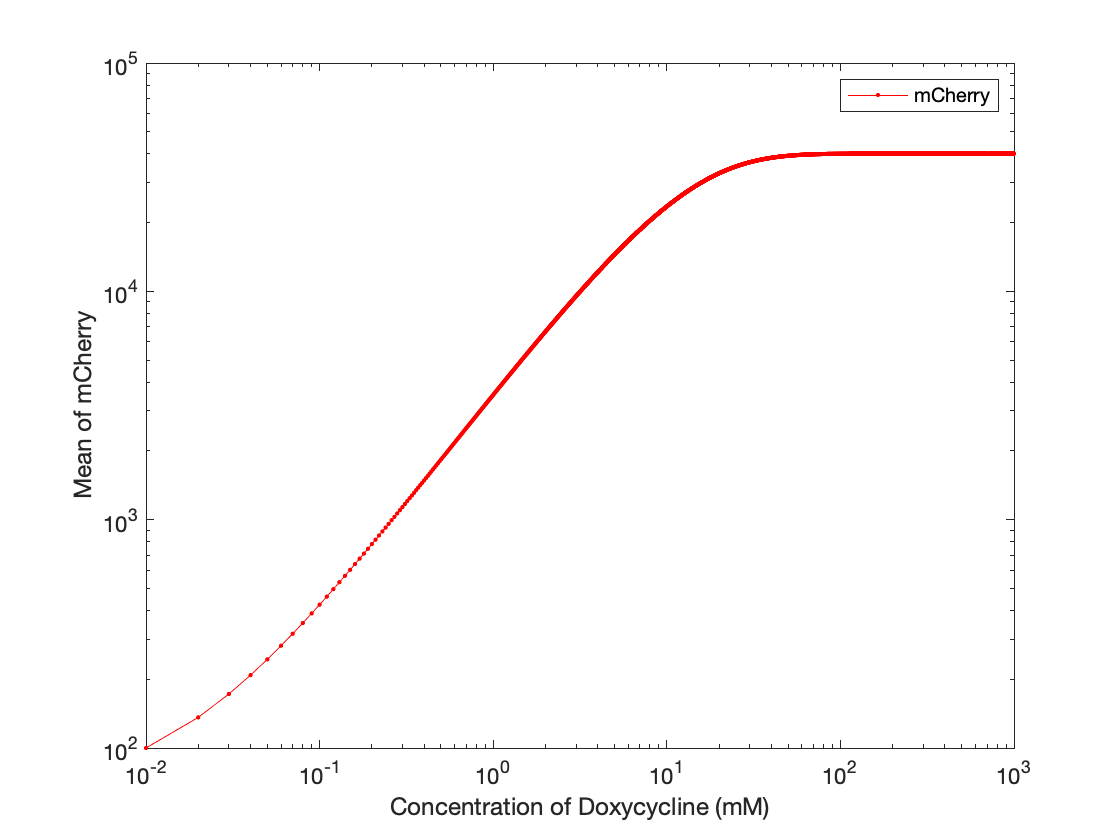
\includegraphics[width=1.0\linewidth]{Figures/Q2_1.png}
\caption{The modeling results for mCherry with feedback}
\label{part_2_model}
\end{figure}

$$K_2 = 1000 mM^{-1}; \sigma_1 = 0.5; K_4 = 0.001 mM^{-1}; \sigma_2 = 0.5;y_0 = 100mM;[R^2_0]_0 = 1000mM$$ 
$$\alpha_1 = 4000 ;\alpha_2 = 4000 ; kdc = 0.01h^{-1} ; kdrd = 0.005h^{-1} ; rc = 10mM*h^{-1} ; rrd = 10mM*h^{-1}$$



%----------------------------------------------------------------------------------------
\newpage
\section{Discuss the differences between Figures \ref{part_2_qestion_figure} F and \ref{part_1_qestion_figure} C, and explain them using the model}

Both the fluorescence of GFP with no feedback and the fluorescence of mCherry with feedback are increased when the concentration of Doxycycline increased. But the processes are quite different.

For the modeling results for GFP with no feedback (shown as Figure 1.2), The slope of curve is changed, it is larger when the Dox concentration is near 1$mM$ while is smaller in two side. Without feedback, the increasing GFP expression does not influencing the system itself. So that there is a threshold for concentration of Dox, when it reaches the threshold, the expression level of the target increases rapidly until the limit is reached.

For the modeling results for mCherry with feedback(shown as Figure 2.2), The slope of the curve is nearly unchanged, so it seems to be a line, which means the expression of mCherry is much more relates to the concentration of Dox. With feedback, the influence of dox is sensed, and the increasing tetR expression inhibits its own expression by binding to the promoter. The expression of the mCherry increases slowly, due to the suppression, and it’s more stable and was directly changed by Dox.



  
\chapter{Modeling  the heterogeneity of the Dox-induced GFP (or mCherry) expressions} % Main chapter title

\label{Part3_chapter} % For referencing the chapter elsewhere, use \ref{Chapter1} 

\section{The model}
In order to access the heterogeneity of Dox-induced single-cell expressions in both feedback and no-feedback systems, we model the random fluctuation in biochemical reactions, random copy number variation and random epigenetic inheritance in expression systems.

\subsection{Random epigenetic inheritance}

Random epigenetic inheritance also plays an important part of fluctuation in cell population. I incorporate random epigenetic inheritance on single cell level. Epigenetic regulations, including DNA methylation, histone modification and others, influence gene expression by regulating chromatin accessibility and the interaction between DNA and protein. In the model, the reaction constants of each transcription was influenced by a random variable $\mu$ which subscribes to normal distribution.

Where:

\begin{equation} 
\begin{aligned} 
\centering
% \underset{A}{B}
% \overset{…}{…}
K_{real}   &= K_{deterministic} \times (1+\mu_1) \\
k_{d-real} &= k_{d-deterministic} \times (1+\mu_2) \\
r_{real}   &= r_{deterministic} \times (1+\mu_3) \\
\beta_{real}   &= \beta_{deterministic} \times (1+\mu_4) \\
\end{aligned} 
\end{equation}

\subsection{Random copy number variance}

Random copy number variance is an important source of noise in cell population. We incorporate random copy number variation on single cell level. In the modeling, the copy number was considered in the $\alpha$, which was influenced by a random variable $\tau$ which subscribes to normal distribution.

Where:

\begin{equation} 
\begin{aligned} 
\centering
% \underset{A}{B}
% \overset{…}{…}
\alpha_{real}   &= \alpha_{deterministic} \times (1+\tau) \\
\end{aligned} 
\end{equation}

\subsection{Random basal expression level of GFP, mCherry and tetR-dimer}

Random copy number variance is an important source of noise in cell population. We incorporate random copy number variation on single cell level. In the modeling, the basal expression level of GFP, mCherry and free tetR-dimer were influenced by a random variable $\xi$ which subscribes to normal distribution.

Where:

\begin{equation} 
\begin{aligned} 
\centering
% \underset{A}{B}
% \overset{…}{…}
[GFP]_{0-real}   &= [GFP]_{0-deterministic} \times (1+\xi_1) \\
[mCherry]_{0-real}   &= [mCherry]_{0-deterministic} \times (1+\xi_2) \\
[R^2_0]_{0-real}   &= [R^2_0]_{0-deterministic} \times (1+\xi_3) \\
\end{aligned} 
\end{equation}

%----------------------------------------------------------------------------------------
\section{Simulate the flow cytometry data with simulations of 1000 cells}

Combing the factors of random fluctuation in biochemical reactions, random copy number variance and random epigenetic inheritance described above, we establish model to study the heterogeneity of Dox-induced single-cell expressions in both feedback and no-feedback systems. For each doxycycline concentration, we stimulate 1000 single cells.

\subsection{Heterogeneity of Dox-induced single-cell expressions, without feedback}

For the heterogeneity of Dox-induced single-cell expressions of GFP without feedback, the stimulation result is as follows:

\begin{figure}[H]
\centering
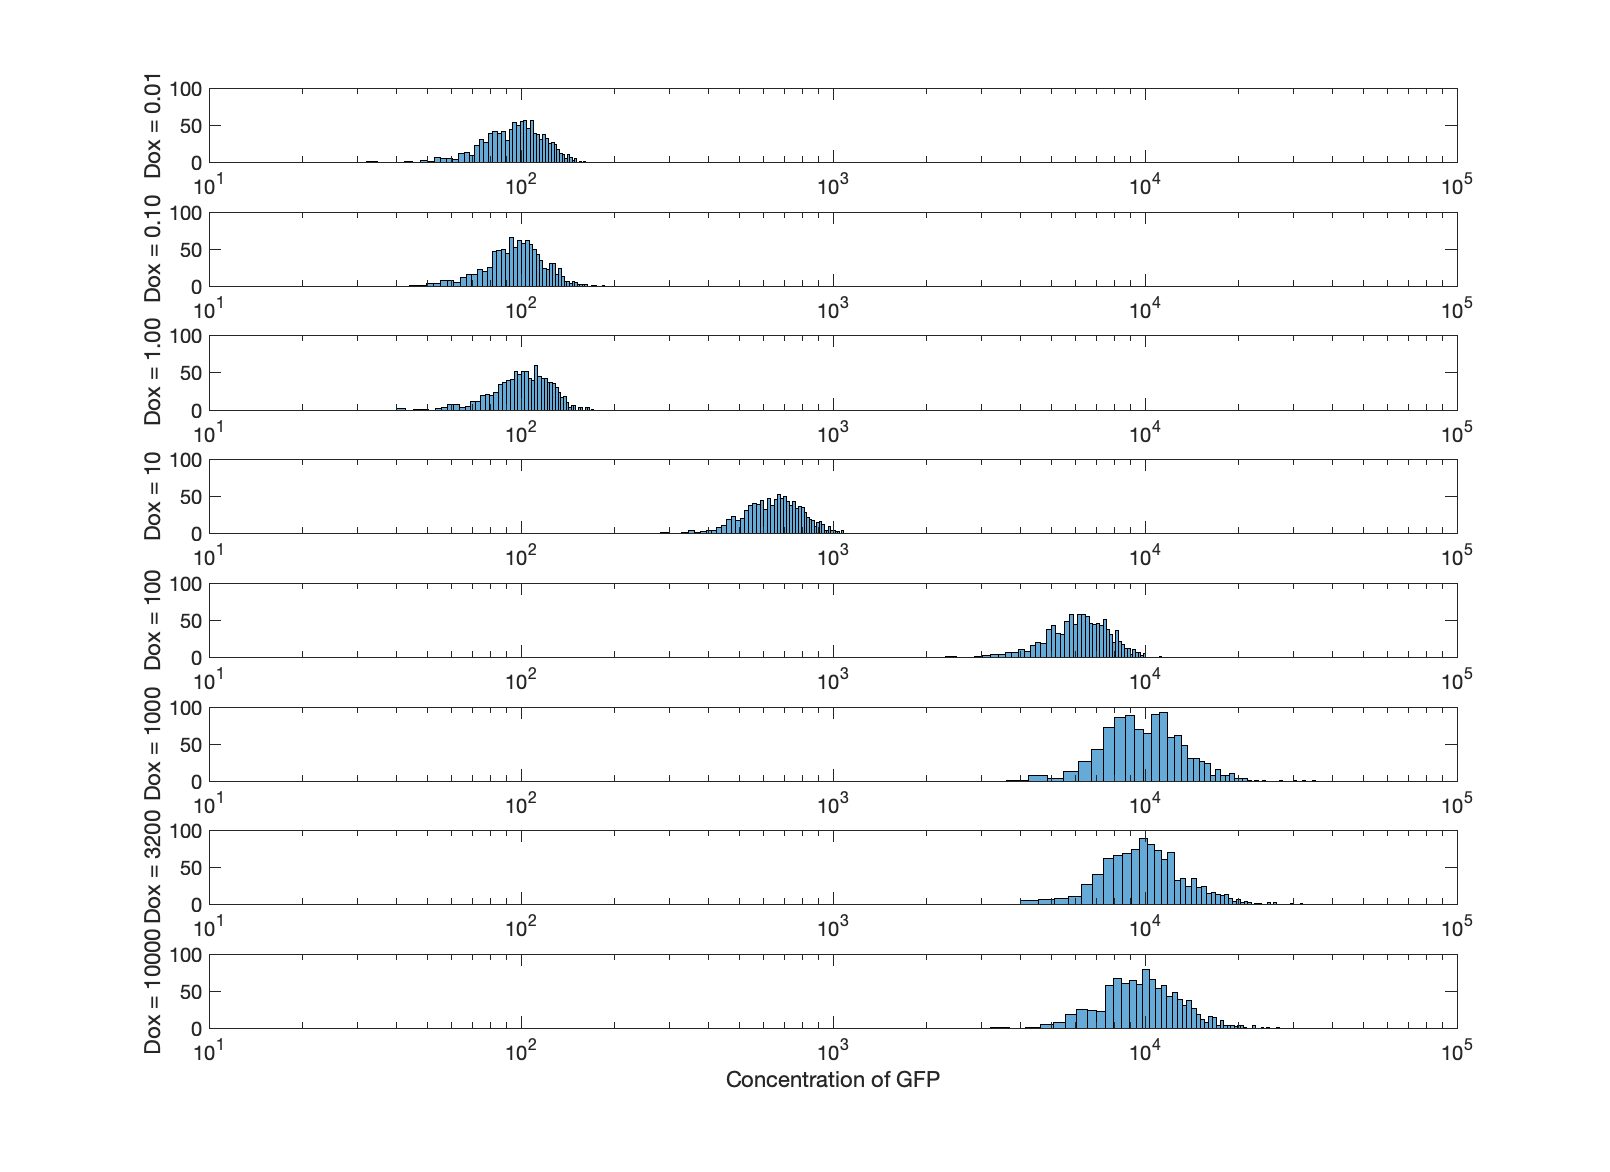
\includegraphics[width=1.0\linewidth]{Figures/Q3_1.png}
\caption{Cytometry simulations of Dox-induced GFP expression \\ system without feedback in 1000 cells}
\label{part_3_1}
\end{figure}

From the figure we can see that for each concentration of doxycycline, the GFP expression in cell population is like a normal distribution. At low concentration of doxycycline, increasing doxycycline concentration would not cause much to distribution of GFP expression, this is because at this stage there is surplus of tetR dimer in addition to binding most of tetO. At higher concentration of doxycycline, increasing doxycycline concentration would not cause much change to the distribution of GFP expression, this is because at this stage the doxycycline is enough to bind most of the tetR dimer.

\subsection{Heterogeneity of Dox-induced single-cell expressions, with feedback}

For the heterogeneity of Dox-induced single-cell expressions of mCherry with feedback, the result is as follows:

\begin{figure}[H]
\centering
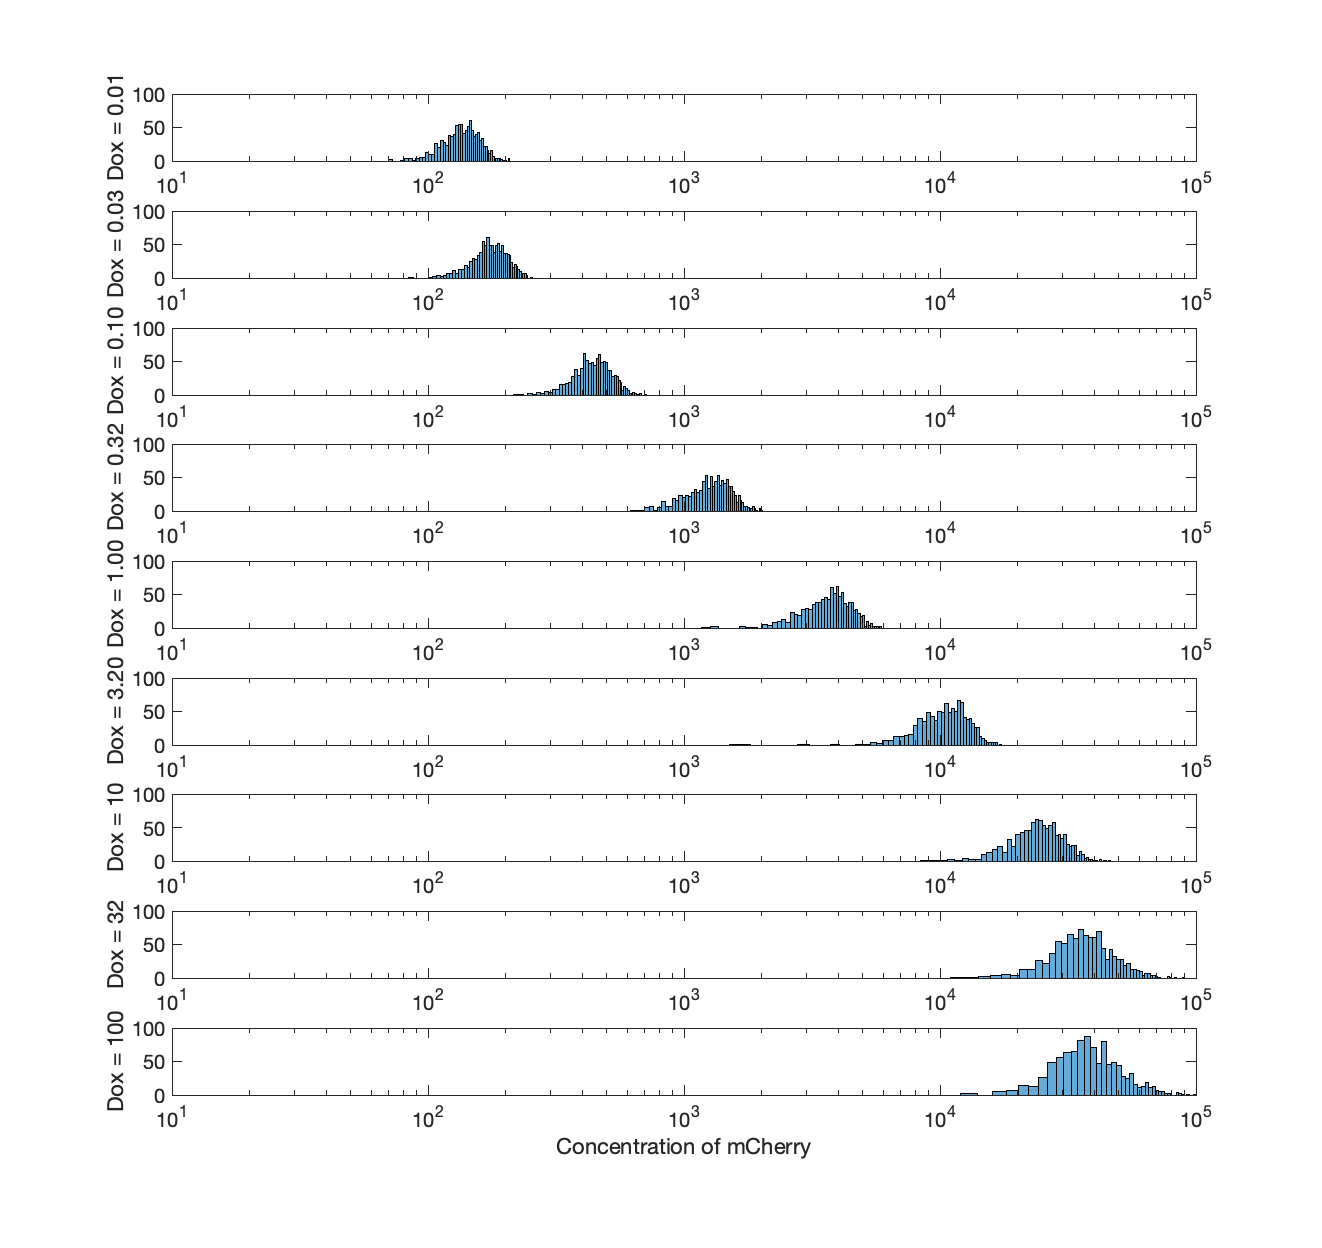
\includegraphics[width=1.0\linewidth]{Figures/Q3_2.png}
\caption{Cytometry simulations of Dox-induced mCherry expression \\system with feedback in 1000 cells ($log10 \approx 3.2$)}
\label{part_3_2}
\end{figure}

From the figure we can see that for each concentration of doxycycline, the mCherry expression in cell population is like a normal distribution. As the concentration of doxycycline increase, the mean of mCherry expression show a steady increase. This is because there is a negative feedback control loop in this system, increasing the concentration of doxycycline will always lead to the system to reach a new equilibrium.

%----------------------------------------------------------------------------------------
\newpage
\section{Discussion}
In this session, we discuss the result and compare our results with the experiment result.

For part1, our result looks very similar to the experiment result, including the initial value, the end value and the turning point. At low concentration of doxycycline, increasing doxycycline concentration would not cause much difference to GFP expression, this is because at this stage there is surplus of tetR dimer in addition to binding most of tetO. At higher concentration of doxycycline, increasing doxycycline concentration would not cause much to GFP expression too, this is because at this stage the doxycycline is enough to bind most of the tetR dimer. This system is responsive to doxycycline only in a narrow range of doxycycline concentration, and the response is ultrasensitive.

For part2, our result also looks very alike to the experiment result, including the initial value and the end value. As the concentration of doxycycline increase, the mean of mCherry expression show a steady increase. This is because there is a negative feedback control loop in this system, increasing the concentration of doxycycline will always lead to the system to reach a new equilibrium. This system is sensitive to a wide range doxycycline and it is easy to tune to achieve precise and quantitate control mCherry expression.

We combine the result of part1 and part2 together, the result is as follows:

\begin{figure}[H]
\centering
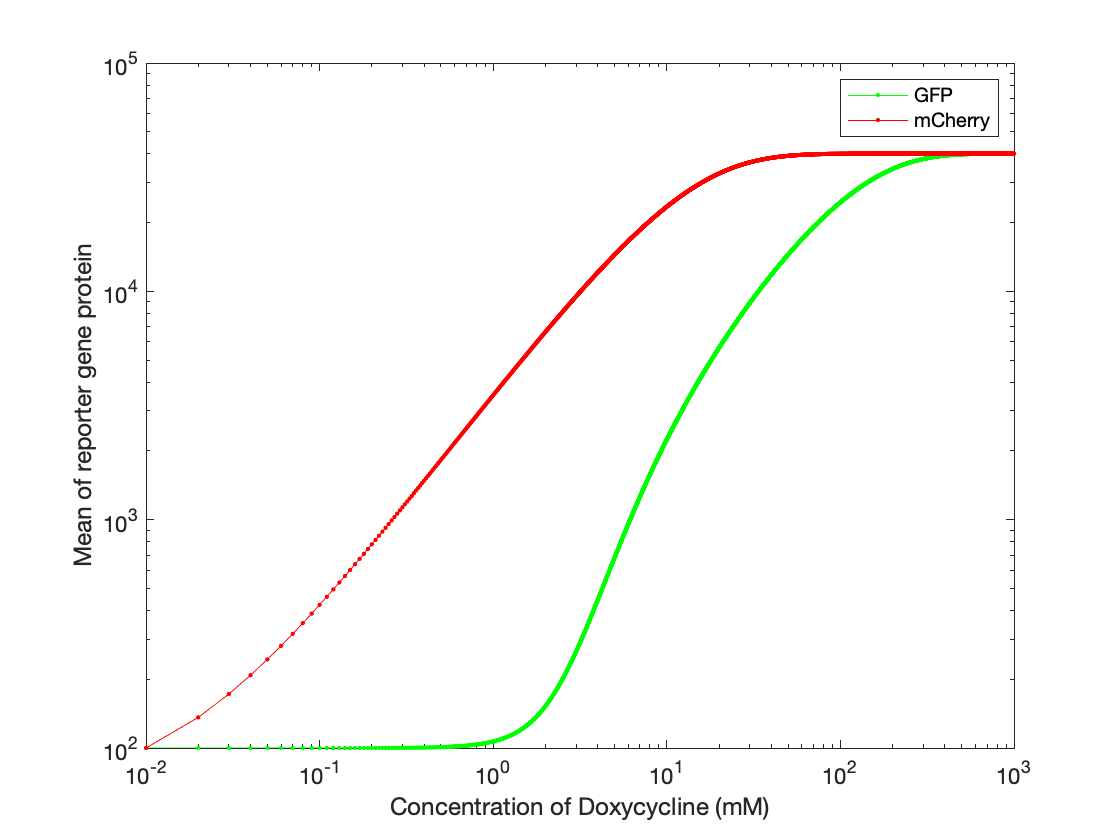
\includegraphics[width=0.8\linewidth]{Figures/Q3_3.png}
\caption{The modeling results for GFP without feedback \\ and mCherry with feedback}
\label{part_3_3}
\end{figure}

The system without feedback is ultrasensitive to doxycycline in a narrow concentration range, while the system with feedback is sensitive to a wide range doxycycline and it is easy to tune to achieve precise and quantitate control mCherry expression. The difference is due to the feedback control: It can control the equilibrium of the reaction and stabilize the system, thus the system with feedback is responsive to wider range of doxycycline concentration, and increasing the concentration of doxycycline will lead to gentle change in target gene expression.

For part3, our modeling result of the system without feedback has similar mean value of the distribution comparing with the experiment result. But at higher concentration of doxycycline, the distribution of experiment result has heavier tail than our modeling result. We hypothesis that the difference is due to some unknown biological pathways. For instance, at higher concentration of doxycycline, some other biological pathways are affected thus lead to the heavier tail in the distribution of experiment result. In addition, our modeling result of system with feedback is similar to the experiment result, both in mean value and distribution shape.


%\include{Chapters/Chapter4} 
%\include{Chapters/Chapter5} 


%	THESIS CONTENT - APPENDICES
 

\appendix % Cue to tell LaTeX that the following "chapters" are Appendices

% Include the appendices of the thesis as separate files from the Appendices folder
% Uncomment the lines as you write the Appendices

%% Appendix A

\chapter{Frequently Asked Questions} % Main appendix title

\label{AppendixA} % For referencing this appendix elsewhere, use \ref{AppendixA}

\section{How do I change the colors of links?}

The color of links can be changed to your liking using:

{\small\verb!\hypersetup{urlcolor=red}!}, or

{\small\verb!\hypersetup{citecolor=green}!}, or

{\small\verb!\hypersetup{allcolor=blue}!}.

\noindent If you want to completely hide the links, you can use:

{\small\verb!\hypersetup{allcolors=.}!}, or even better: 

{\small\verb!\hypersetup{hidelinks}!}.

\noindent If you want to have obvious links in the PDF but not the printed text, use:

{\small\verb!\hypersetup{colorlinks=false}!}.

%\include{Appendices/AppendixB}
%\include{Appendices/AppendixC}

 
%	BIBLIOGRAPHY
 
\renewcommand*{\bibfont}{\fontsize{9pt}{8pt} \selectfont}
\printbibliography[heading=bibintoc]
\end{document}  
